\chapter{Wymagania niefunkcjonalne}
\section{Środowisko uruchomieniowe}
	\begin{itemize}
		\item System operacyjny Linux
			\begin{itemize}
				\item Dystrybucje:
				\begin{itemize}
					\item Manjaro 17.01;
				\end{itemize}
				\item Zależności:
					\begin{itemize}
						\item CMake 3.15.4;
						\item Boost C++ Libraries 1.71;
						\item Git -> Pobranie kodu produkcyjnego, GTest, GMock;
						\item GCC 9.2;
					\end{itemize}
			\end{itemize}
		\item Podłączenie do internetu w celu pobrania repozytorium oraz kompilacji programu uruchomieniowego;
		\item Komendy wywoływane w pierwszym oknie konsoli, w celu uruchomienia symulatora urządzenia:
		\begin{enumerate}
			\item ,,git clone https://github.com/trunksBT/KorytkoMag\_RetSimulator.git -{}-recursive''
			\item ,,cd KorytkoMag\_RetSimulator''
			\item ,,make .''
			\item ,,bash runBinary.sh''
		\end{enumerate}
		\item Komendy wywoływane w drugim oknie konsoli, w celu uruchomienia sterownika urządzenia:
		\begin{enumerate}
			\item ,,git clone https://github.com/trunksBT/KorytkoMag\_RetDriverSimulator.git -{}-recursive''
			\item ,,cd KorytkoMag\_RetDriverSimulator''
			\item ,,make .''
			\item ,,bash runBinary.sh''
			\item Wywołanie komend zgodnie z diagramem sekwencji zatytułowanym ,,KalibracjaRETa''
			\item Aby zakończyć trzeba wpisać ,,exit''
		\end{enumerate}
	\end{itemize}
\section{Zrzuty ekranu}
	\begin{figure}[p]
	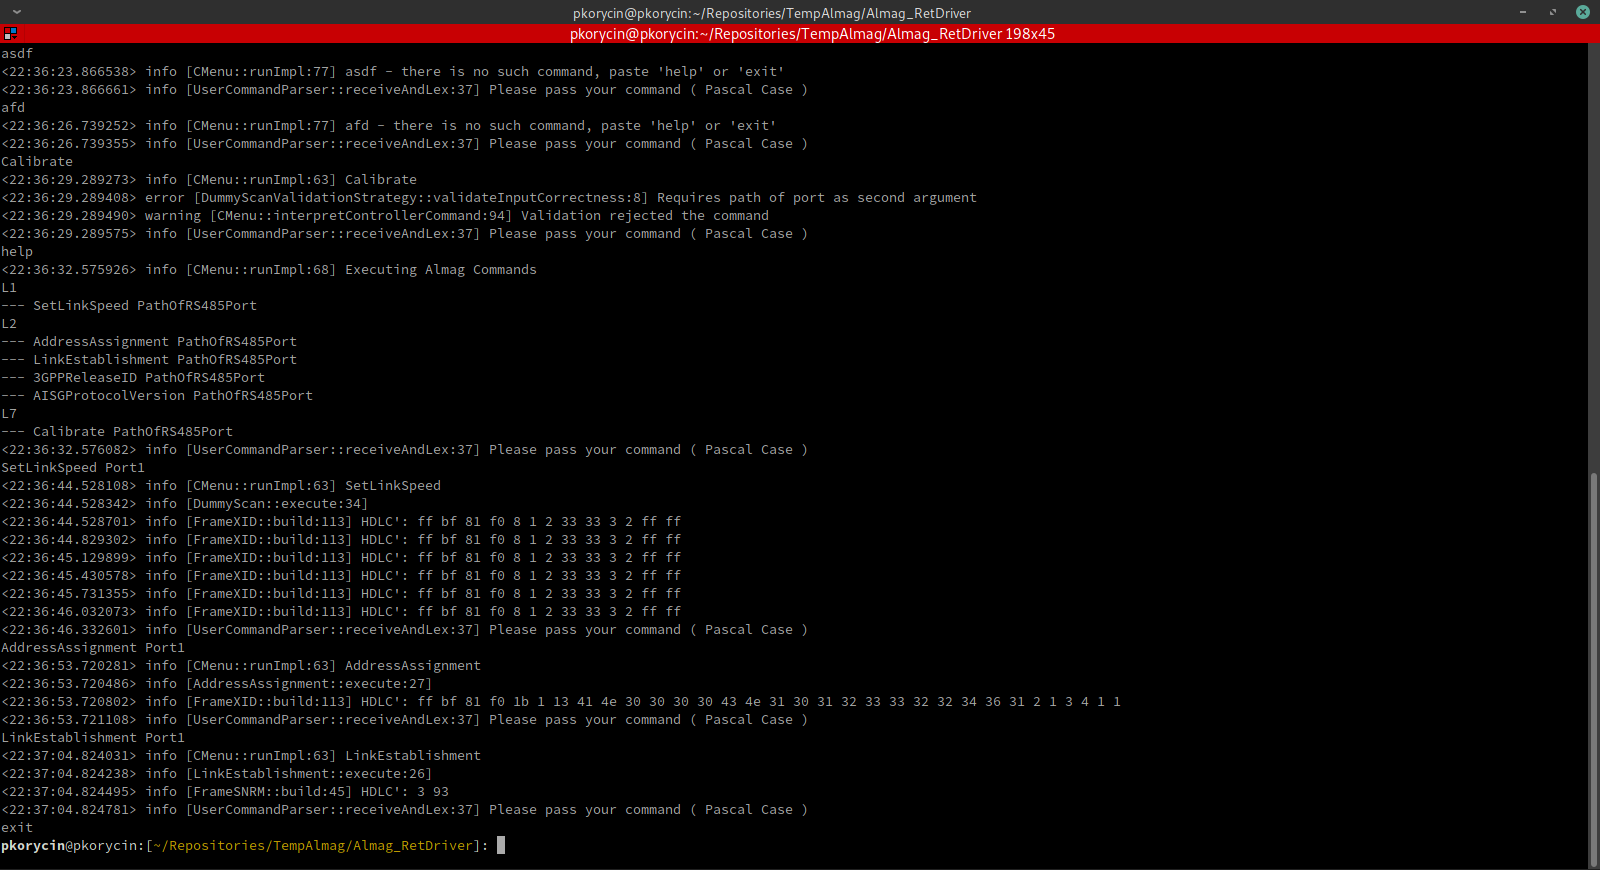
\includegraphics[scale=0.3]{ExecutionOnSeverityInfo.png}
	\caption{Zrzut ekranu z wykonania testów modułowych}
	\end{figure}
	
	\begin{figure}[p]
	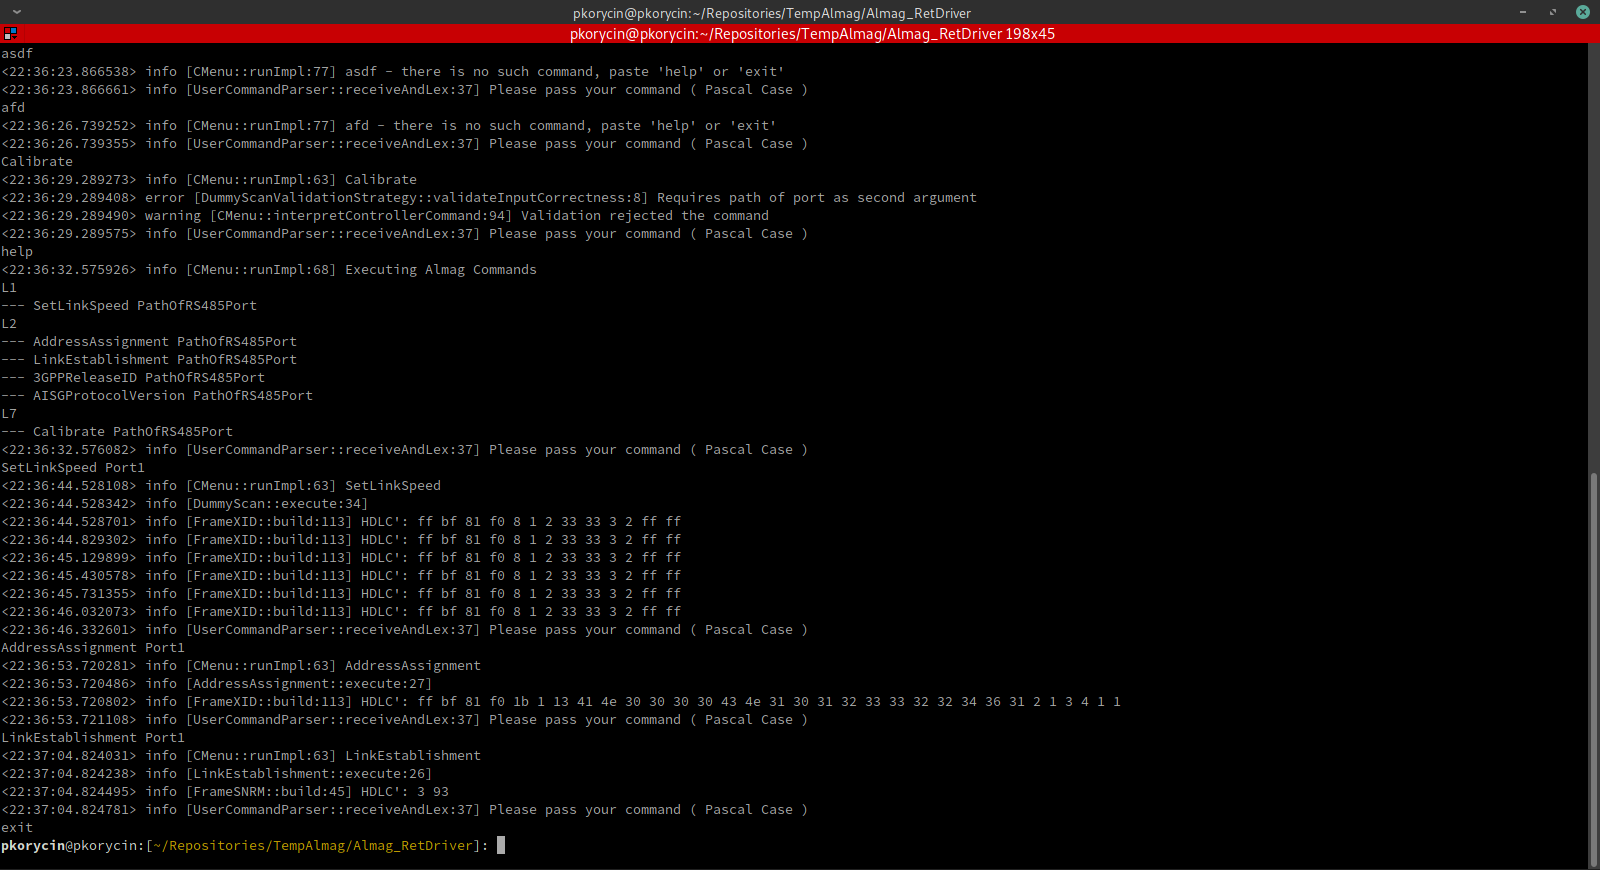
\includegraphics[scale=0.3]{ExecutionOnSeverityInfo.png}
	\caption{Zrzut ekranu z wykonania testów jednostkowych}
	\end{figure}
	
	\begin{figure}[p]
	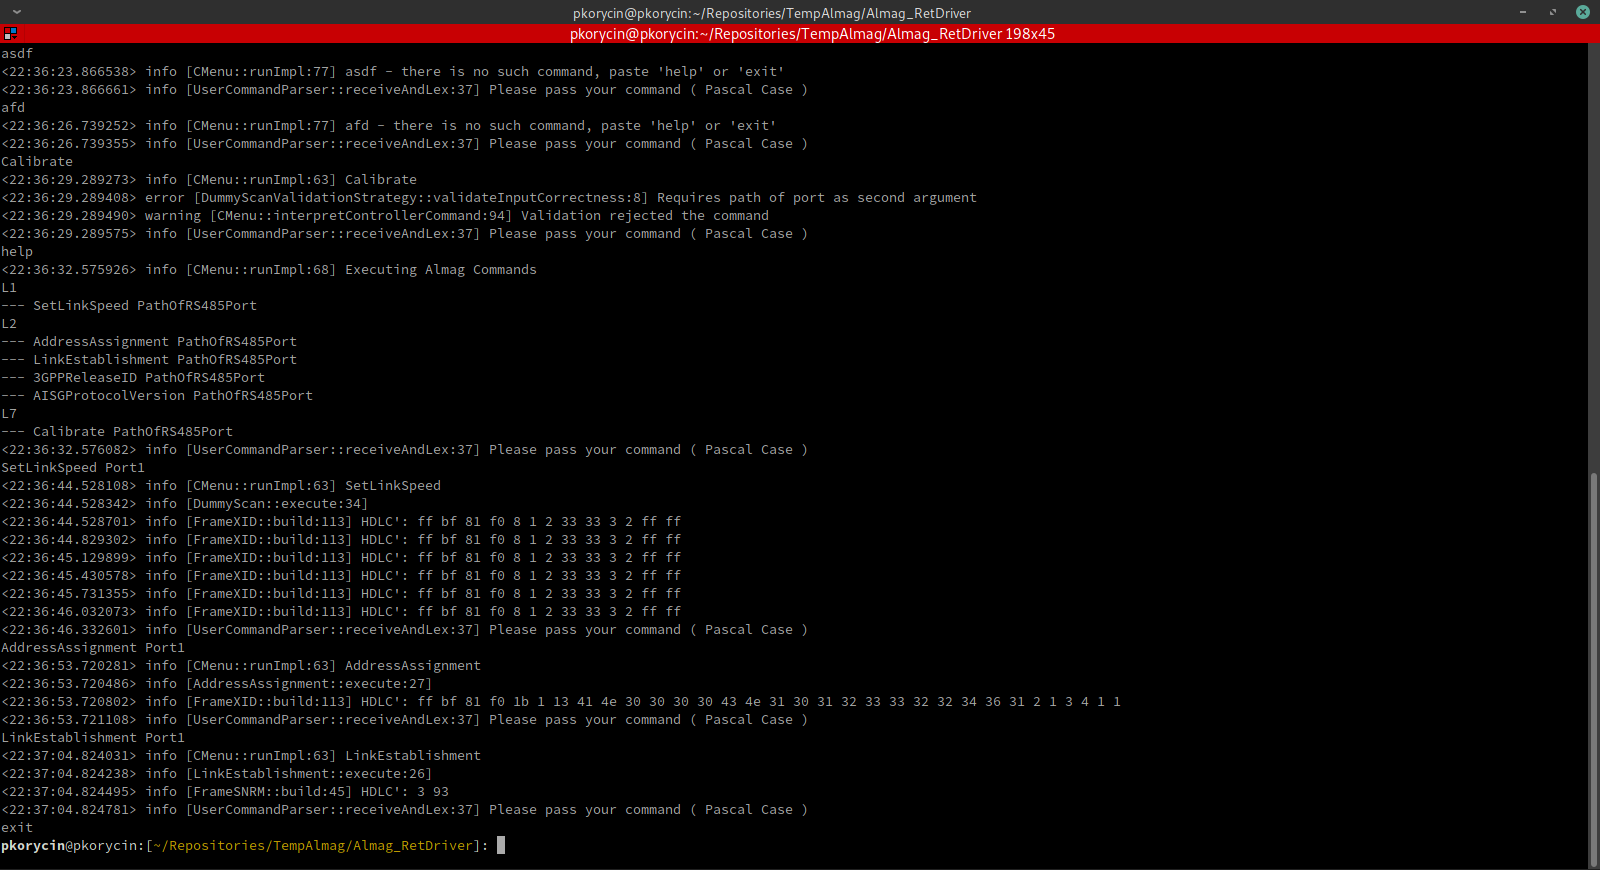
\includegraphics[scale=0.3]{ExecutionOnSeverityInfo.png}
	\caption{Zrzut ekranu z uruchomienia programu z odfiltrowaniem logów poniżej priorytetu info}
	\end{figure}
	
	\begin{figure}[p]
	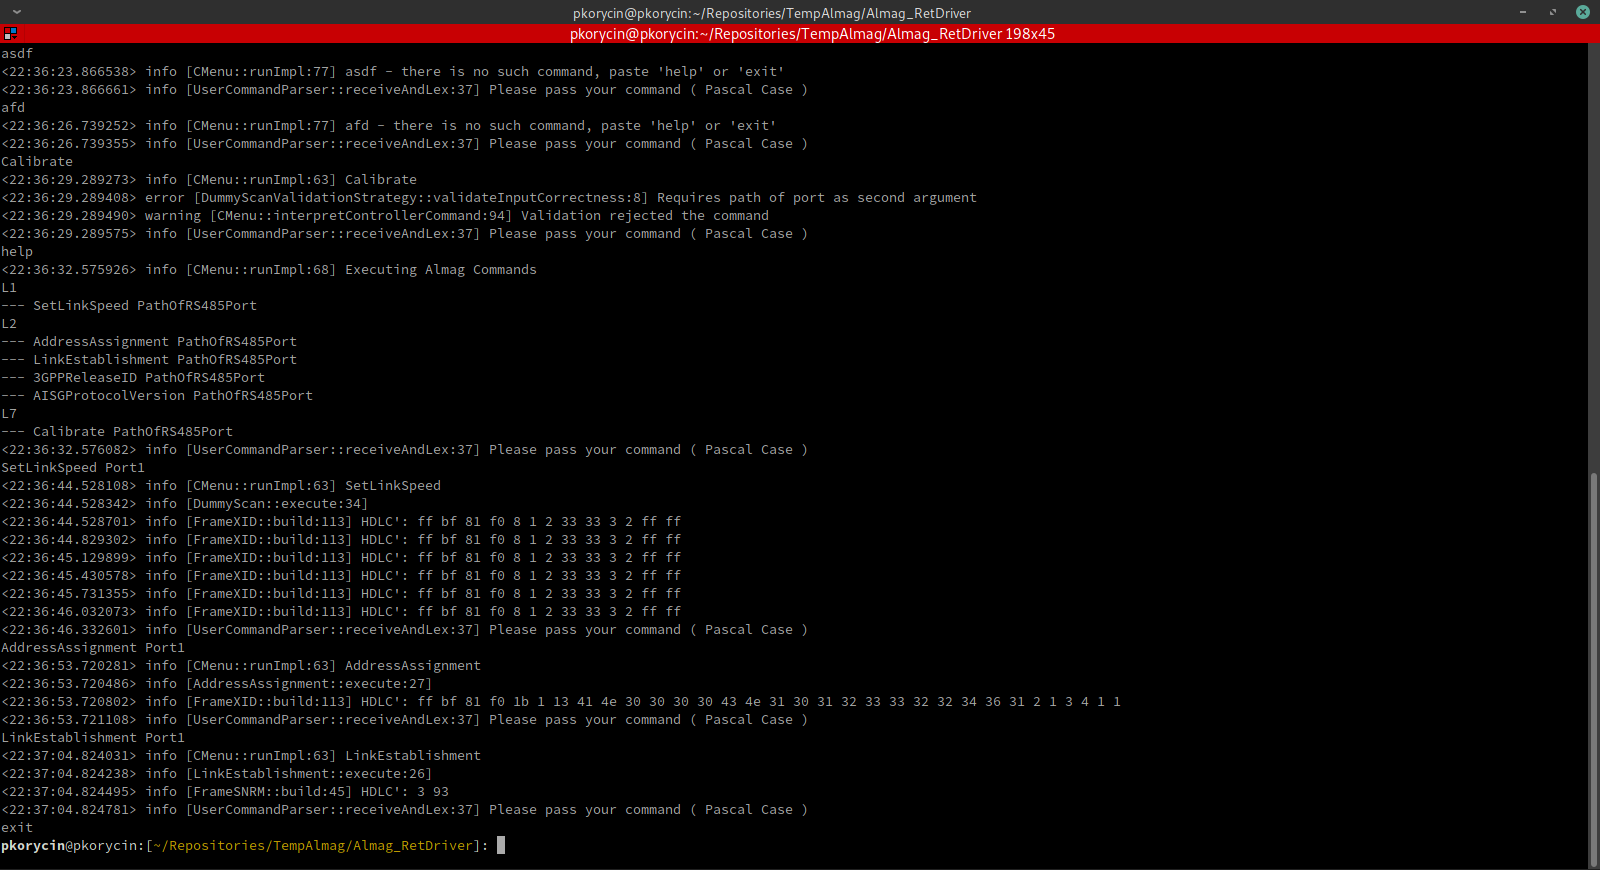
\includegraphics[scale=0.3]{ExecutionOnSeverityInfo.png}
	\caption{Zrzut ekranu z uruchomienia programu bez odfiltrowania logów}
	\end{figure}

